\documentclass{article}
\usepackage{amsmath}
\usepackage{graphicx}
\usepackage{verbatim}
\usepackage{color}   %May be necessary if you want to color links
\usepackage{hyperref}
\usepackage[utf8]{inputenc}
\usepackage{tikz}
\usetikzlibrary{shapes.geometric,arrows}

\tikzstyle{startstop}=[rectangle,rounded corners,minimum width=3cm,
minimum height=1cm,text centered,draw=black,fill=red!30]
\tikzstyle{io}=[trapezium,trapezium left angle=70, trapezium right angle= 110,minimum width=6cm,
minimum height=1cm,text centered,draw=black,fill=blue!30]
\tikzstyle{process}=[rectangle,minimum width=3cm,
minimum height=1cm,text centered,text width=3cm,draw=black,fill=orange!30]
\tikzstyle{decision}=[diamond,minimum width=3cm,
minimum height=1cm,text centered,draw=black,fill=green!30]
\tikzstyle{arrow}=[thick,->,>=stealth]

\hypersetup{
    colorlinks=true, %set true if you want colored links
    linktoc=all,     %set to all if you want both sections and subsections linked
    linkcolor=blue,  %choose some color if you want links to stand out
}
\begin{document}
    \begin{titlepage}
        \begin{center}
            \vspace*{0cm}
            \Huge
            \textbf{ELP780}
     
            \vspace{0.5cm}
            \LARGE
            Software Lab
     
            \vspace{1.5cm}
            \textbf{Aghil Sabu\\}

            \vspace{.3cm}
            2018EET2865
     
            \vfill
            A report presented for the assignment on\\
            Assignment 8 - Python and Github 
     
            \vspace{0.8cm}
            \includegraphics[width=0.45\textwidth]{./images/logo}
     
            \Large
            Electrical Engineering\\
            IIT Delhi\\
            India\\
            \today
        \end{center}
    \end{titlepage}
    \tableofcontents
    \pagenumbering{arabic}
    \pagebreak
    
    \section{Problem Satement 1}
    \subsection{Problem Statement}
    \textbf{Parity Check}
    \\ \\The simplest way of error detection is to append a single bit, called a parity check, to a string of data bits. This parity check bit has the value 1 if the number of 1’s in the bit string is even and has the value 0 otherwise, i.e., Odd Parity Check.\\ \\
    \textbf{Bit-Oriented Framing}
    \\ \\Data Link Layer needs to pack bits into frames so that each frame is distinguishable from another. Frames can be fixed or variable size. In variable size framing, we define the end of the frame using a bit-oriented approach. It uses a special string of bits, called a flag for both idle fills and to indicate the beginning and the ending of frames.\\ 
    The bit stuffing rule is to insert a 0 after each appearance of 010 in the original data. \\
    The string 0101 is used as the bit string or flag to indicate the end of the frame.\\ \\

    \subsection{Input Format}
    Enter binary bit data that has to be transmitted.\\

    \subsection{Output Format}
    Print binary bit data with parity bit.\\
    Print the modified string that is to be transmitted\\   \\

    \subsection{Sample Input}
    010101110100101

    \subsection{Sample Output}
    Parity bit data : 0101011101001011\\
    Transmitting data: 01001011101000100110101

    \subsection{PS1 algorithm}
    \begin{itemize}
        \item Read bit data from user
        \item Initialize parity as 1
        \item XOR parity with all bits to get parity value
        \item append parity bit
        \item replace pattern 010 with 0100
        \item append 0101 at the end
        \item display rsults in the required format
    \end{itemize}
    \subsection{PS1 Flow Chart}
    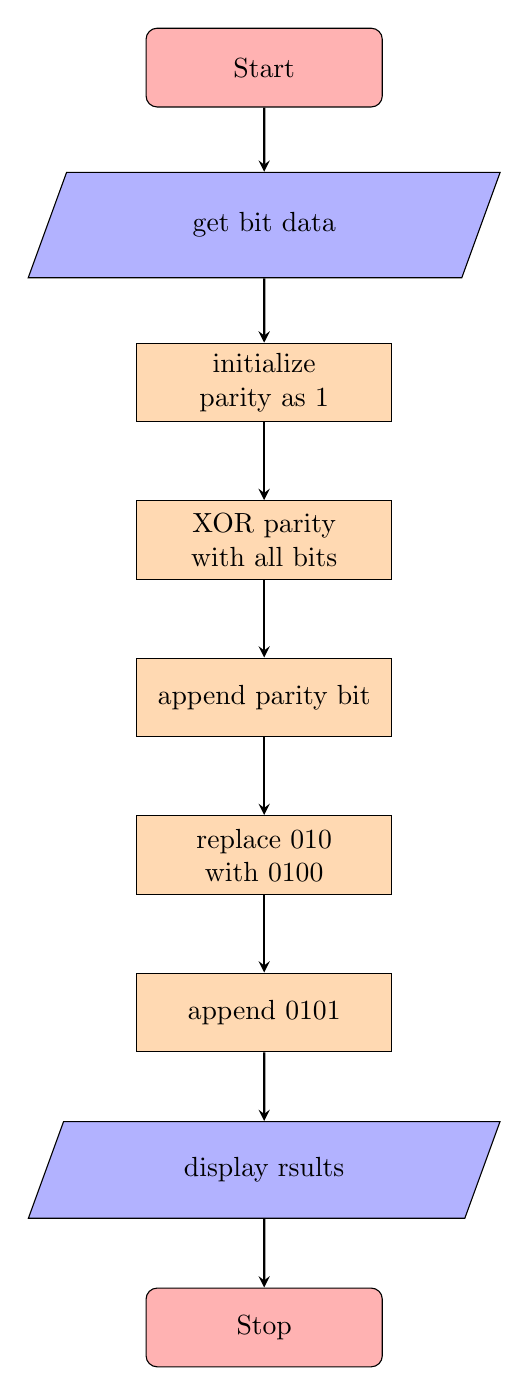
\begin{tikzpicture}[node distance=2cm]
        \node (start) [startstop] {Start};
        \node (p1) [io,below of=start] {get bit data};
        \node (p2) [process,below of=p1] {initialize parity as 1};
        \node (p3) [process,below of=p2] {XOR parity with all bits};
        \node (p4) [process,below of=p3] {append parity bit};
        \node (p5) [process,below of=p4] {replace 010 with 0100};
        \node (p6) [process,below of=p5] {append 0101};
        \node (p7) [io,below of=p6] {display rsults};
        \node (stop) [startstop,below of=p7] {Stop};

    
        \draw [arrow] (start) -- (p1);
        \draw [arrow] (p1) -- (p2);
        \draw [arrow] (p2) -- (p3);
        \draw [arrow] (p3) -- (p4);
        \draw [arrow] (p4) -- (p5);
        \draw [arrow] (p5) -- (p6);
        \draw [arrow] (p6) -- (p7);
        \draw [arrow] (p7) -- (stop);
    
    
    
    \end{tikzpicture}
    \pagebreak
    \subsection{PS1 Solution-Code}
    \verbatiminput{ps1.py}
    
    \pagebreak
    \subsection{PS1 Output Screenshots}
    \begin{center}     
        \includegraphics[width=1.1\textwidth]{./images/ps1_001.png}
    \end{center}
    \pagebreak
    \section{Problem Satement 2}
    A 8085 assembler is designed in a way that it takes input assembly source code instructions in
all capital letters and numbers in hexadecimal format suffixed by H.
You have to create preprocessor for assembler that will translate any 8085 assembly code into
full capital letters and all numerals into hexadecimal format suffixed by H.
Use lex(flex) and Yacc(bison).
        
    \subsection{PS2 algorithm}
    \begin{itemize}
        \item Get filenames from user
        \item for each line get all characters before colon ':'
        \item make all uppercase
        \item add hexadecimal 'H' wherever required
        \item save result to output file
    \end{itemize}
    \subsection{PS2 Flow Chart}
    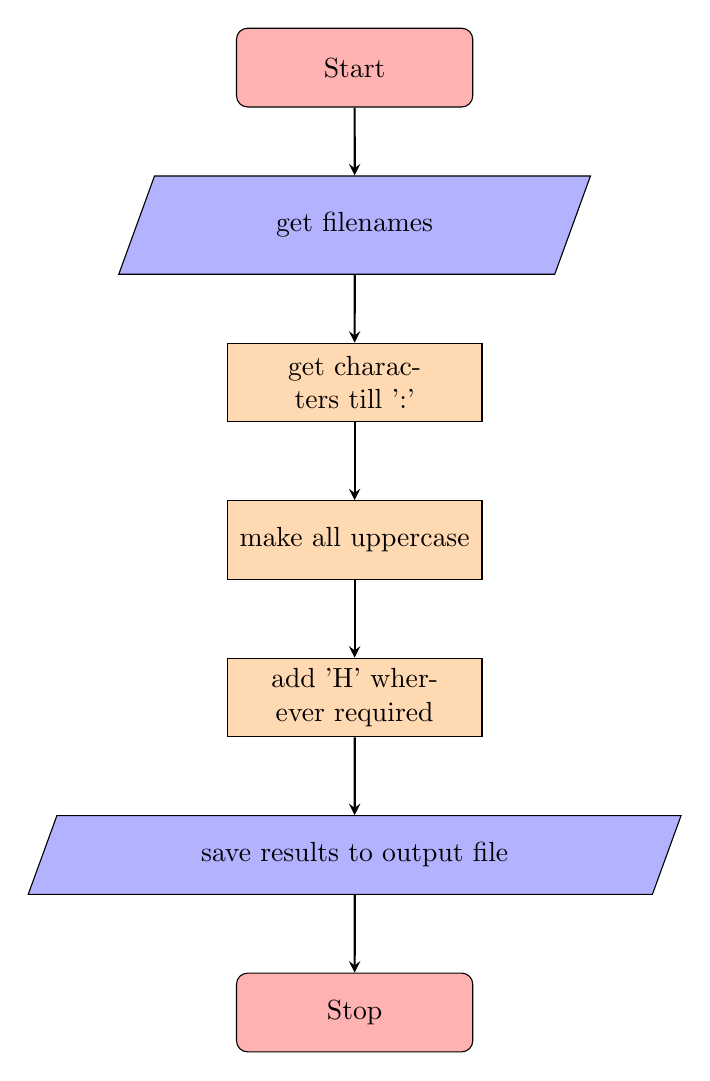
\begin{tikzpicture}[node distance=2cm]
        \node (start) [startstop] {Start};
        \node (p1) [io,below of=start] {get filenames};
        \node (p2) [process,below of=p1] {get characters till ':'};
        \node (p3) [process,below of=p2] {make all uppercase};
        \node (p4) [process,below of=p3] {add 'H' wherever required};
        \node (p5) [io,below of=p4] {save results to output file};
        \node (stop) [startstop,below of=p5] {Stop};

    
        \draw [arrow] (start) -- (p1);
        \draw [arrow] (p1) -- (p2);
        \draw [arrow] (p2) -- (p3);
        \draw [arrow] (p3) -- (p4);
        \draw [arrow] (p4) -- (p5);
        \draw [arrow] (p5) -- (stop);
    
    
    
    \end{tikzpicture}
    \pagebreak
    \subsection{PS2 Solution-Code}
    \verbatiminput{ps2.l}

    \pagebreak
    \subsection{PS2 Output }
    \subsubsection{input file}
    \verbatiminput{ps2.txt}
    \subsubsection{output file}
    \verbatiminput{output.txt}
    % \includegraphics[width=1.2\textwidth]{./images/ps2_001.png}
    \pagebreak
    \section{makefile}
    \subsection{makefile code}
    \verbatiminput{makefile}
    % \subsection{makefile Screenshots}
    % \includegraphics[width=1.2\textwidth]{./images/mk_001.png}
    \subsection{makefile output}
    \includegraphics[width=1.2\textwidth]{./images/mk_001.png}


    \section{GIT}
    \subsection{GIT Commit Screenshots}
    \includegraphics[width=1.2\textwidth]{./images/gt_001.png}
    \includegraphics[width=1.2\textwidth]{./images/gt_001.png}

\end{document}